\chapter{Photon Interaction Cross Sections and Sampling Techniques}
\label{ch:photon_interactions}
In the previous two chapters, the Monte Carlo random walk process for both
neutral and charged radiation was described. An important part of the random
walk process is the indirect sampling of the collision kernel, which requires
information on the differential interaction cross sections for the particle
of interest. In this chapter, four primary interactions of high energy photons 
with matter will be discussed: incoherent scattering, coherent scattering, 
pair production and the photoelectric effect. Photonuclear absorption, which can
become important in high energy coupled neutron-photon transport simulations, 
will be discussed briefly. In addition, sampling procedures that can be used 
with each differential interaction cross section will be discribed. All 
secondary particles other than photons will be neglected from the cross sections
and sampling procedures. 

\section{Incoherent Scattering}
Incoherent or Compton scattering occurs when a photon scatters off of an orbital
electron and loses some of its energy. The energy of the liberated electron
is equal to the energy lost by the photon minus the binding energy of the
shell the electron occupied. The differential incoherent scattering cross
section (per atom) is usually expressed as the product of the differential 
Klein-Nishina scattering cross section per electron and the incoherent 
scattering function. Klein and Nishina developed the differential cross section
under the assumption that the electron on which the photon scatters is free 
and at rest \citep{klein_uber_1929}. The incoherent scattering function is the 
correction to the Klein-Nishina scattering cross section from electron binding. 
The differential incoherent scattering cross section is shown below 
\citep{lux_monte_1991}. The value $r_e^2$ is the classical radius of the 
electron and $\alpha^{'}$ is the energy of the incident photon in units of 
electron rest energy.
\begin{align}
  \frac{d\sigma_{i.s.}(\alpha^{'},\theta,Z)}{d\Omega} & = 
  \frac{d\sigma_{K.N.}(\alpha^{'},\theta)}{d\Omega}S(y,Z) \nonumber \\
  & = \frac{r_e^2}{2}
  \frac{\left[1 + \cos{^{2}\theta} + \frac{\alpha^{'2}(1-\cos{\theta})^2}
                                  {1 + \alpha^{'}(1-\cos{\theta})}\right] }
  {\left[1 + \alpha^{'}(1-\cos{\theta}) \right]^2}
  S(y,Z)
  \label{eq:incoh_scat_theta}
\end{align}
The arguments of the scattering function are 
$y = sin(\frac{\theta}{2})/\lambda^{'}$ and $Z$, the atomic number. The 
differential incoherent cross section will sometimes be expressed in terms of 
the outgoing photon energy as well. The alpha variables are simply the photon
energy divided by the rest mass of the electron.
\begin{equation}
  \frac{d\sigma_{i.s.}(\alpha^{'},\theta,Z)}{d\Omega} = \frac{r_e^2}{2}
  \left(\frac{\alpha}{\alpha^{'}} \right)^2
  \left[ \frac{\alpha}{\alpha^{'}} + \frac{\alpha^{'}}{\alpha} - 1 + 
    \cos{^2\theta} \right] S(y,Z)
\end{equation}
The later form of the differential incoherent cross section is made possible 
by the one-to-one correspondance between the outgoing energy and outgoing 
direction, which can be found using conservation of energy and momentum and the 
assumption that the electron is free and at rest (see Appendix 
\ref{ch:appendix_B}). 
\begin{equation}
  E = \frac{E^{'}}{1 + \frac{E^{'}}{m_ec^2}(1 - \cos{\theta})}
  \label{eq:compton_scattering_energy_rel}
\end{equation}
When binding effects cannot be neglected, which typically occurs when the 
incident photon energies are on the order of the electron binding energy, there 
will no longer be a one-to-one correspondance between the outgoing energy and 
the outgoing direction. Instead, there will be a distribution of outgoing 
energies that correspond to each outgoing direction. This phenomenon will be 
discussed more in the next section.

A PDF for the outgoing photon angle can be created by dividing the differential
incoherent cross section by the total incoherent cross section at the incoming
photon energy. Then, by reorganizing the PDF, the procedure for sampling an
outgoing photon direction and energy can be determined 
\citep{persliden_monte_1983}.
\begin{align}
  p(\alpha^{'},\theta,Z) & = \frac{1}{\sigma_{i.s.}(\alpha^{'},Z)}
  \frac{d\sigma_{i.s.}(\alpha^{'},\theta,Z)}{d\Omega} \nonumber \\
  & = \frac{S_{max}(y,Z) \sigma_{K.N.}(\alpha^{'})}{\sigma_{i.s.}(\alpha^{'},Z)}
  \left[ \frac{S(y,Z)}{S_{max}(y,Z)} \right]
  \left[ \frac{1}{\sigma_{K.N.}(\alpha^{'})} 
    \frac{d\sigma_{K.N.}(\alpha^{'},\theta)}
         {d\Omega} \right] \nonumber \\
  & = C(\alpha^{'},Z) R(y,Z) p_{K.N.}(\alpha^{'},\theta) 
  \label{eq:incoherent_sampling_pdf}
\end{align}
The scattering function increases monotonically from 0 when $y=0$ to Z when
$y=\infty$ and therefore,
\begin{equation*} 
S_{max}(y,Z) = S(y_{max},Z).
\end{equation*}
The maximum value of $y$, which occurs when $\theta = \pi$ (corresponding to
back scattering), is simply the inverse wavelength of the incoming 
particle (usually in $cm^{-1}$). Now, to sample the outgoing direction, one 
first samples an angle from the PDF for Compton Scattering off of a free 
electron, $p_{K.N.}(\alpha,\theta)$. Then one uses the rejection function R(y,Z)
with the sampled angle to determine if it should be accepted or rejected. 
Several sampling techniques that can be used with the Klein-Nishina cross 
section will now be discussed.

For the purpose of sampling, it is useful to write the differential 
Klein-Nishina cross section in terms of a new variable whose inverse is the 
energy loss ratio.
\begin{align}
  \frac{1}{x} & = \frac{\alpha}{\alpha^{'}} \\
  x = 1+\alpha^{'}(1-\cos{\theta})
\end{align}
The differential Klein-Nishina cross section can then be written as follows 
\citep{lux_monte_1991}.
\begin{align}
  \frac{d\sigma_{K.N.}(\alpha^{'},x)}{dx} & = K \left[ A + \frac{B}{x} +
    \frac{C}{x^2} + \frac{D}{x^3} \right] \\
  K & = \frac{\pi r_e^2}{\alpha^{'}} \nonumber \\
  A & = \frac{1}{\alpha^{'2}} \nonumber \\
  B & = 1 - \frac{2(\alpha^{'} + 1)}{\alpha^{'2}} \nonumber \\
  C & = \frac{1 + 2\alpha^{'}}{\alpha^{'2}} \nonumber \\
  D & = 1 \nonumber
\end{align}
The change of variables is carried out in Appendix \ref{ch:appendix_B}.

Now, a PDF for $x$ can be created if the differential Klein-Nishina cross 
section is divided by the total Klein-Nishina cross section, which can be found 
by integrating the differential Klein-Nishina cross section from $x_{min} = 1$ to
$x_{max} = 1 + 2 \alpha^{'}$\footnote{The equation found in Lux and Koblinger's
text book contains an error which is described in Appendix \ref{ch:appendix_B}}.
\begin{equation}
  \sigma_{K.N.}(\alpha^{'}) = 2\pi r_e^2 \left( \frac{1+\alpha^{'}}{\alpha^{'2}}
  \left[\frac{2+2\alpha^{'}}{1+2\alpha^{'}} - 
    \frac{ln(1+2\alpha^{'})}{\alpha^{'}} \right]
  + \frac{ln(1+2\alpha^{'})}{2\alpha^{'}} - 
  \frac{1+3\alpha^{'}}{(1+2\alpha^{'})^2} \right)
\end{equation}
At low photon energies, the evaluation of this equation for the Klein-Nishina 
cross sections can lead to numerical errors due to the near-cancellation between
logarithmic and algebraic terms \citep{lux_monte_1991}. An empirical formula
was created that is correct to within $1.3\%$ up to 100 MeV
\citep{hastings_approximations_1955}. Due to the sampling techniques that will
be used, the total Klein-Nishina cross section will only need to be evaluated
when the incoming photon energy is above about $1.4$ MeV. Therefore there is no 
need to use the empirical formula.

The PDF for $x$ can be defined as follows.
\begin{align}
  p_{K.N.}(\alpha^{'},x) & = 
  \begin{cases}
    H \cdot \left[ A + \frac{B}{x} + \frac{C}{x^2} + \frac{D}{x^3} \right]
    & \text{if } 1 \leq x \leq 1 + 2 \alpha^{'} \\
    0 & \text{o.w.}
  \end{cases} \\
  H & = \frac{K}{\sigma_{K.N.}(\alpha^{'})} \nonumber 
\end{align}
A direct inversion of this PDF is not possible. However, this PDF can still be
sampled directly by using a combination of the probability mixing method and the
inverse CDF method \citep{koblinger_direct_1975}\footnote{For a description of 
all sampling methods that one can use, please refer to refs. \citep{koblinger_direct_1975, lux_monte_1991, spanier_monte_1969, blomquist_assessment_1983}.}. To
use these two sampling techniques, the PDF must be split into four terms. 
\begin{align}
  p_{K.N.}(\alpha^{'},x) = p_1(\alpha^{'},x) + p_2&(\alpha^{'},x) +
  p_3(\alpha^{'},x) + p_4(\alpha^{'},x) \\
  p_1(\alpha^{'},x) & = HA \nonumber \\
  p_2(\alpha^{'},x) & = \frac{HB}{x} \nonumber \\
  p_3(\alpha^{'},x) & = \frac{HC}{x^2} \nonumber \\
  p_4(\alpha^{'},x) & = \frac{HD}{x^3} \nonumber 
\end{align}
Now the $i^{th}$ term can be selected with the following probability.
\begin{equation}
  p_i = \int_1^{1+2\alpha^{'}} p_i(\alpha^{'},x) dx
\end{equation}
For the four functions above, the probabilities of being selected are shown
below. Take note that these probabilities contain the total Klein-Nishina
cross section.
\begin{equation}
  p_i = 
  \begin{cases}
    \frac{2H}{\alpha^{'}} & \text{if } i = 1 \\
    H \left[1 - \frac{2+2\alpha^{'}}{\alpha^{'2}} \right] ln(1 + 2\alpha^{'}) 
    & \text{if } i = 2 \\
    \frac{2H}{\alpha^{'}} & \text{if } i = 3 \\
    \frac{H}{2} \left[1 - \frac{1}{(1+2\alpha^{'})^2} \right] & \text{if } i = 4
    \end{cases}
\end{equation}
In order for this method to work, all of the probabilities must be positive.
Therefore, $p_2$ and $p_4$ impose limits on the values of $\alpha^{'}$ where this
method can be used. The probability $p_2$ is the more restrictive of the two.
When the value of $\alpha^{'}$ is less than $(1 + \sqrt{3})$, $p_2$ will be 
negative and the method cannot be used. This corresponds to a photon energy of
about $1.4$ MeV. Below this energy another method must be used, which will be 
discussed shortly. Once an $i$ has been selected, the value of $x$ is sampled
from the inverse CDF of $p_i(\alpha^{'},x)$. The inverse CDFs for each of the
four functions is shown below. The uniform random number in the interval (0,1)
required by the inverse CDF method is represented by the variable 
$\varepsilon$.
\begin{align}
  P_1^{-1}(\alpha^{'},\varepsilon) & = 1 + 2\alpha^{'}\varepsilon \\
  P_2^{-1}(\alpha^{'},\varepsilon) & = (1 + 2\alpha^{'})^{\varepsilon} \\
  P_3^{-1}(\alpha^{'},\varepsilon) & = \frac{1 + 2\alpha^{'}}
  {1 + 2\alpha^{'}\varepsilon} \\
  P_4^{-1}(\alpha^{'},\varepsilon) & = \left[1 - \varepsilon\left(1 - 
    \frac{1}{(1 + 2\alpha^{'})^2} \right) \right]^{-\frac{1}{2}}
\end{align}
Evaluating the inverse CDF with a random number yields a value of x from the
Klein-Nishina differential cross section. The value of x can then be used to
determine the new energy and direction (relative to the current direction) of 
the photon.
\begin{align}
  \alpha & = \frac{\alpha^{'}}{x} \\
  \cos{\theta} & = 1 + \frac{1-x}{\alpha^{'}} 
\end{align}

When the energy of the incoming photon drops below 1.4 MeV, the rejection
method can be used to sample values of x from the Klein-Nishina cross section.
Kahn developed a rejection sampling procedure that can be used for any incoming
photon energy. However the efficiency of the procedure is highest at lower 
energies \citep{lux_monte_1991, kahn_applications_1956}. This procedure is
shown in figure \ref{fig:kahn_rejection_sampling}.
\begin{figure}[t!]
  \begin{center}
    \def\svgwidth{300bp}
    \input{chapters/photon_interactions/Kahn_sampling_method.pdf_tex}
  \end{center}
  \caption{\textbf{Kahn's Rejection Sampling Procedure}.
    \textit{This sampling procedure is used to sample a value of x from the
    differential Klein-Nishina cross section. One can use this sampling
    procedure at any incoming particle energy, however the efficiency of the
    procedure degrades at higher enegies \citep{lux_monte_1991}.}}
  \label{fig:kahn_rejection_sampling}
\end{figure}

When the direct sampling method and the rejection method are used together, one 
can efficiently sample values from the Klein-Nishina cross section at any 
incoming photon energy. Figure \ref{fig:diff_KN_sampling_proc_eff} shows the 
efficiency of both Kahn's rejection sampling procedure and the combined 
sampling procedure. At around 1.4 MeV, the efficiency of the combined sampling 
procedure jumps to one because of the switch to the direct sampling method. 
This is a considerable improvement compared to only using Kahn's method.
\begin{figure}[t!]
  \begin{center}
    \scalebox{1.0}{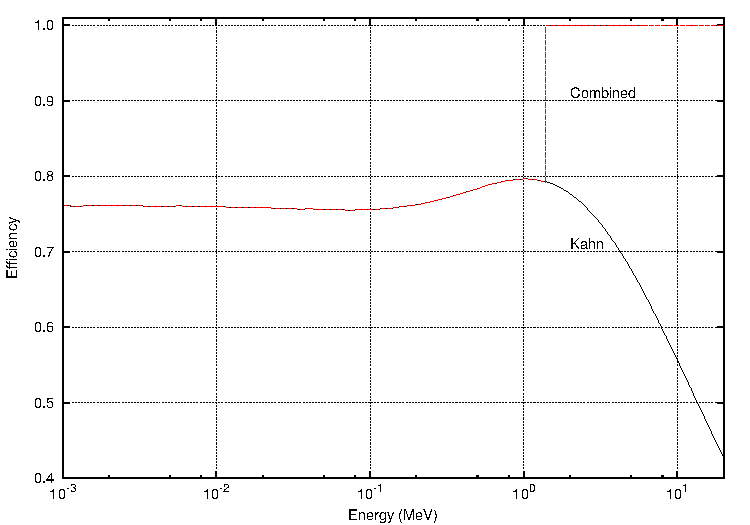
\includegraphics{chapters/photon_interactions/Kahn_Koblinger_sampling_eff_no_binding.pdf}}
  \end{center}
  \caption{\textbf{Differential Klein-Nishina cross section sampling procedure efficiencies.}
    \textit{The efficiency of Kahn's rejection sampling procedure is shown for 
      energies between one keV and twenty MeV. The efficiency of this procedure
      begins to decline around a few MeV. When it is combined with Koblinger's
      direct sampling method, which can only be used above about 1.4 MeV, a
      very efficient sampling method is obtained for all photon energies.}}
  \label{fig:diff_KN_sampling_proc_eff}
\end{figure}

Once an outgoing angle and energy have been selected from the PDF corresponding
to the differential Klein-Nishina cross section, the rejection function 
$R(y,Z)$ from equation \ref{eq:incoherent_sampling_pdf} must be used to 
determine if the outgoing energy and angle should be kept. This rejection 
function will affect the efficiency of the overall sampling procedure 
described by equation \ref{eq:incoherent_sampling_pdf}. Figure 
\ref{fig:diff_incoh_sampling_proc_eff} shows the efficiency of the overall 
sampling procedure for a free electron, Aluminum and Lead. For lower energies 
and higher atomic numbers, the rejection function causes a large decrease in 
the efficiency of the sampling procedure compared to the free electron case 
(where the rejection function is equal to unity at all energies).
\begin{figure}[t!]
  \begin{center}
    \scalebox{1.0}{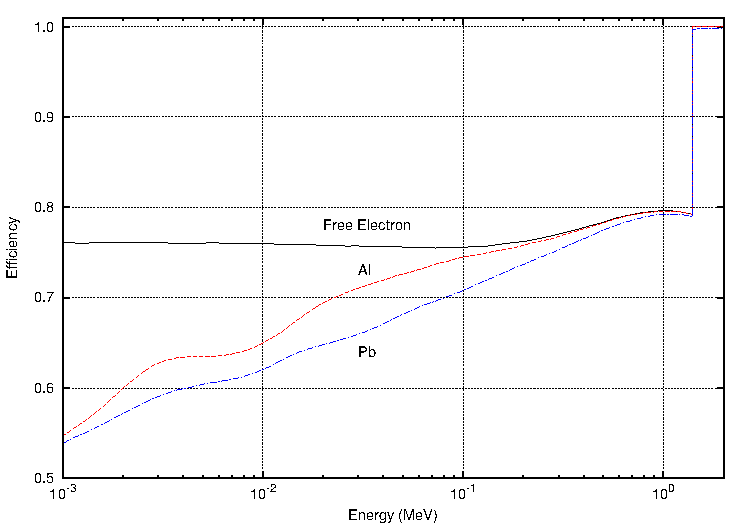
\includegraphics{chapters/photon_interactions/Kahn_Koblinger_sampling_eff.pdf}}
  \end{center}
  \caption{\textbf{Differential incoherent cross section sampling procedure efficiency.}
    \textit{The efficiency of the combined method for sampling from the 
      differential Klein-Nisha cross section with the subsequent evaluation of 
      the rejection function (based on the scattering function) is shown. At
      lower energies and higher atomic numbers, the rejection function has
      a more deleterious effect on the sampling efficiency compared to the 
      free electron case.}}
  \label{fig:diff_incoh_sampling_proc_eff}
\end{figure}

\section{Doppler Broadening of Incoherently Scattered Photons}
\label{sec:photon_dopp_broadening}
As mentioned in the previous section, the differential Klein-Nishina cross 
section assumes that the electron upon which the photon scatters is free
and at rest. Atomic electrons are bound and consequently cannot be at rest. 
When the energy of the incoming photon is much greater than the binding 
energies of the electrons in the atom, binding effects are negligable and the
incoherent cross section becomes simply the atomic number times the 
Klein-Nishina cross section. However, when the incoming photon energy is on the
order of a few hundred keV or lower, binding effects must be taken into account
\citep{namito_implementation_1994}. Taking binding effects into account results
in three significant changes to the simulated transport process. First, electron
binding results in a reduction in the total incoherent cross section, which
in turn results in larger mean free paths for the photon as it travels through
the medium. This occurs because part of the differential cross section is
suppressed because it would result in energetically impossible scattering 
events\footnote{Because the atomic system is a quantum-mechanical system, enough
energy must be given to the electron to free it. Otherwise a reaction will not
occur}. Second, the angular distribution of the scattered photon is 
modified, particurily in the forward direction. Finaly, the Compton-scattered
photon energy is broadened by the pre-collision motion of the electron 
\citep{namito_implementation_1994}. In other words, the one-to-one 
correspondence between the outgoing photon direction and energy is broken and 
for each outgoing direction, there is an associated distribution of outgoing 
photon energies. The first two changes were taken into account in the last
section by multiplying the differential Klein-Nishina cross section by the 
scattering function. In this section, the energy distribution will be dealt
with. 

To take into account the energy distribution, the double differential
incoherent scattering cross section must be used. Using the Born and impulse
approximations, Ribberfors was able to derive the double differential
incoherent scattering cross section, which is shown below 
\citep{ribberfors_x-ray_1983}. This double differential cross section is given 
for each subshell of the atom. The value $\alpha_c$ is called the Compton line, 
which is the outgoing photon energy (divided by the electron rest mass) 
corresponding to the outgoing scattering angle assuming that the electron was 
stationary and free. The variable $\alpha$ is the true outgoing photon 
energy resulting from the collision with a bound, moving electron.
\begin{equation}
  \left(\frac{d^2\sigma(\alpha,\alpha^{'},\theta,Z)}{d\Omega dE}\right)_i = 
  \frac{r_e^2}{2c\left|\vec{\alpha^{'}} - 
    \vec{\alpha}\right|} \left(\frac{\alpha}{\alpha^{'}}\right) 
  \left(\frac{\alpha^{'}}{\alpha_c} + \frac{\alpha_c}{\alpha^{'}} - 1 + 
  cos^2\theta \right) J_i(p_z,Z)
\end{equation}
The function $J_i(p_z,Z)$ is the Compton profile for the $i^{th}$ electron 
subshell for element $Z$. The argument $p_z$ is the projection of the 
electron's initial momentum on the scattering vector 
$\vec{\alpha^{'}} - \vec{\alpha}$. Because of the quantum mechanical nature of 
the atomic system, the electrons in each subshell have an associated 
probability distribution in momentum space, which is often denoted 
$n_i(\vec{p},Z)$. The Compton profile is simply the projection of this 
probability distribution along the scattering vector 
\citep{cooper_compton_1985}.
\begin{equation}
  J_i(p_z,Z) = \int_{p_x} \int_{p_y} n_i(p_x,p_y,p_z,Z)dp_xdp_y
\end{equation}

For the purposes of sampling from this double differential cross section it
will be more useful to do a change of variables from outgoing energy to 
electron momentum projection $p_z$. Using conservation of energy and momentum,
an equation for the electron momentum projection can be determined. This
derivation is shown in Appendix \ref{ch:appendix_B}. 
\begin{align}
  p_z & = m_ec \frac{\alpha - \alpha^{'} + \alpha^{'}\alpha(1 - \cos{\theta})}
  {\left|\vec{\alpha^{'}} - \vec{\alpha}\right|} \nonumber \\
  & = m_ec \frac{\alpha - \alpha^{'} + \alpha^{'}\alpha(1 - \cos{\theta})}
  {\sqrt{\alpha^{'2} + \alpha^{2} - 2\alpha^{'}\alpha^{'2}cos{\theta}}}
  \label{eq:pz}
\end{align}
The derivative of this equation with respect to the outgoing photon energy
is shown below.
\begin{equation}
  \frac{dp_z}{d\alpha} = m_ec \frac{1 + \alpha^{'}(1-\cos{\theta})}
  {\left|\vec{\alpha^{'}} - \vec{\alpha} \right|} - 
  p_z \frac{\left(\alpha - \alpha^{'}\cos{\theta} \right)}
  {\left|\vec{\alpha^{'}} - \vec{\alpha} \right|^2}
  \label{eq:diff_pz}
\end{equation}
Ribborfors suggested a simplification to this derivative based on some 
observations about the Compton profiles \citep{ribberfors_x-ray_1983}. First, 
the Compton profiles are even functions. Therefore, the odd moments of $p_z$ 
will be zero. Second, the Compton profiles drop off fairly rapidly so that
the first moment can be approximated as follows. The limit of integration
$p_{i,max}$ will be explained shortly.
\begin{equation}
  \langle p_z \rangle \approx \int_{-\infty}^{p_{i,max}} p_z J(p_z)dp_z = 0
\end{equation}
Therefore, the second term in equation \ref{eq:diff_pz} can be ignored because
it will not contribute significantly to the total incoherent cross section\footnote{In the change of variables $\frac{d\alpha}{dp_z}$ is used. However, 
constructing a Maclaurin series in $p_z$ to first order will give the same result.}.
\begin{align}
  \frac{dp_z}{d\alpha} & = m_ec \frac{1 + \alpha^{'}(1-\cos{\theta})}
  {\left|\vec{\alpha^{'}} - \vec{\alpha} \right|} \nonumber \\
  & = \frac{m_ec \alpha^{'}}
  {\alpha_c \left|\vec{\alpha^{'}} - \vec{\alpha} \right|}
  \label{eq:diff_pz_simp}
\end{align}
Now the change of variables in the double differential cross section can be
completed \citep{ribberfors_x-ray_1983}.
\begin{align}
  \left(\frac{d^2\sigma(p_z,\theta,Z)}{d\Omega dp_z}\right)_i & = 
  \left(\frac{d^2\sigma(\alpha,\alpha^{'},\theta,Z)}{d\Omega dE}\right)_i 
  \frac{dE}{d\alpha}
  \frac{d\alpha}{dp_z} \nonumber \\ 
  & =  \frac{r_e^2}{2} \left(\frac{\alpha\alpha_c}{\alpha^{'2}}\right) 
  \left(\frac{\alpha^{'}}{\alpha_c} + \frac{\alpha_c}{\alpha^{'}} - 1 + 
  cos^2\theta \right) J_i(p_z,Z)
\end{align}

The differential incoherent scattering cross section from the previous section
can be recovered by integrating over all possible electron momentum projections
and by summing up the resulting differential cross section for each shell.
Because $\alpha$ and $p_z$ are related by equation \ref{eq:pz}, this integral
will be quite complicated. Fortunately, Ribberfors has shown that using the
approximation $\alpha_c \approx \alpha$ results in negligable errors in the 
total incoherent scattering cross section \citep{ribberfors_x-ray_1983}. The
limit of integration $p_{i,max}$ is the maximum electron momentum projection
allowed for a compton scattering reaction to occur. This maximum occurs when
the outgoing photon energy is equal to $E - E_{i,b}$, where $E_{i,b}$ is the 
binding energy for the particular subshell. Unfortunately, $p_{i,max}$ is a 
function of $\theta$ so this integral will still be complicated. 
\begin{align}
  \frac{d\sigma_{i.s.}(\alpha^{'},\theta,Z)}{d\Omega} & = 
  \frac{r_e^2}{2} \left(\frac{\alpha_c}{\alpha^{'}}\right)^2 
  \left(\frac{\alpha^{'}}{\alpha_c} + \frac{\alpha_c}{\alpha^{'}} - 1 + 
  cos^2\theta \right) \sum_i \int_{-\infty}^{p_{i,max}} J_i(p_z,Z)dp_z \nonumber \\
  & = \frac{d\sigma_{K.N.}(\alpha^{'},\theta)}{d\Omega} S^I(y,Z) \nonumber \\
  & = \frac{d\sigma_{K.N.}(\alpha^{'},\theta)}{d\Omega} S(y,Z) \nonumber
\end{align}

The scattering function $S^I(y,Z)$ is the scattering function from the
impulse approximation. The scattering function that is given in most tables
and is recommended for use in Monte Carlo codes is based on the Waller-Hartree
theory. Both of these scattering functions have been shown to be in close 
agreement for many elements though, which is why a direct substitution is 
justified \citep{namito_implementation_1994}. 

The method proposed by Namito et al. for sampling an outgoing photon energy
from the double differential incoherent cross section will now be discussed
\citep{namito_implementation_1994}. The first step is to sample an outgoing
scattering angle from the differential incoherent cross section using the 
methods from the previous section. Next, the subshell containing the electron 
upon which the photon will scatter must be sampled. The most accurate
way to sample the subshell would be to create a discrete PDF based on the total
incoherent cross section for each subshell. This data isn't readily available in
the popular tables \citep{cullen_epdl97_1997}. The approximation used by Namito 
et al., which is only truely applicable when the incoming photon energy is much 
greater than the binding energy of the electron, is to sample the electron shell
based on the number of electrons present in each shell (given as $n_i$).
\begin{align}
  p(i) & = \frac{(\sigma_{i.c.})_i}{\sigma_{i.c.}} \nonumber \\
  & \approx \frac{\sigma_{K.N.}n_i}{\sigma_{K.N.}Z} \nonumber \\
  & \approx \frac{n_i}{Z} 
\end{align}
Finally, an outgoing photon energy must be sampled from the double differential 
incoherent cross section. A conditional PDF for the outgoing photon energy can 
be created by dividing the double differential incoherent cross section by the 
differential incoherent cross section evaluated at a particular angle. The value
of $p_{i,max}$ is calculated from the equation for $p_z$ using the value of 
$\theta$ that was sampled and the substitution 
$\alpha = \alpha^{'}-\frac{E_{i,b}}{m_ec^2}$.
\begin{align}
  p_i(p_z,Z \text{ | } \theta) & = 
  \left(\frac{d\sigma_{i.s.}(\alpha^{'},\theta,Z)}{d\Omega} \right)_i^{-1}
  \left(\frac{d^2\sigma(\alpha,\alpha^{'},\theta,Z)}{d\Omega dp_z}\right)_i 
  \nonumber \\
  & = \left(\frac{\alpha_c\alpha}{\alpha^{'2}}\right)
  \left(\frac{\alpha^{'}}{\alpha_c}\right)^2
  \frac{J_i(p_z,Z)}{S_i(y,Z)} \nonumber \\
  & = (1 + \alpha^{'}\cos{\theta})\left(\frac{\alpha}{\alpha^{'}}\right)
  \left(\frac{J_i(p_z,Z)}{\int_{-\infty}^{p_{i,max}}J_i(p_z,Z)dp_z}\right) \nonumber\\
  & = C(\alpha^{'},\theta)R(\alpha,\alpha^{'})p(p_z,Z)
\end{align}
One must sample a value of $p_z$ from the PDF $p(p_z,Z)$ to determine the
outgoing photon energy. Once the outgoing photon energy has been determined
the rejection function $R(\alpha,\alpha^{'})$ is used to determine if the value 
should be accepted or rejected. The CDF corresponding to the PDF for $p_z$ is 
the following\footnote{Namito et al. actually recommend the CDF $\frac{\int_{0}^{p_z}J_i(x,Z)dx}{\int_{0}^{p_{i,max}}J_i(x,Z)dx}$, which appears to be an error.}.
\begin{equation}
P(p_z,Z) = \frac{\int_{-\infty}^{p_z}J_i(x,Z)dx}{\int_{-\infty}^{p_{i,max}}J_i(x,Z)dx}
\end{equation}
Because the Compton profiles are most commonly found in tabular form\footnote{Biggs et al. have compiled the Compton profiles for atomic numbers 1-102\citep{biggs_hartree-fock_1975}.}, a table method must be used to sample the value of 
$p_z$. One first finds the value of the CDF corresponding to the momentum 
projection $p_{i,max}$. Then one finds the momentum projection associated with 
the CDF value $\varepsilon\int_{-\infty}^{p_{i,max}}J_i(x,Z)dx$, where $\varepsilon$ 
is again a uniform random number. Using a standard binary search algorithm, 
this process can be done very efficiently.

The equation for the outgoing photon energy in terms of the momentum projection
is shown below. When both values are energetically possible, one of the values
must be randomly selected (with probability one half).
\begin{align}
  \alpha & = \frac{-b}{2a} \pm \frac{\sqrt{b^2 - 4ac}}{2a} \\
  a & = \left(\frac{p_z}{m_ec}\right)^2 - 
  \left(\frac{\alpha^{'}}{\alpha_c}\right)^2
  \nonumber \\
  b & = -2\alpha^{'}\left[\left(\frac{p_z}{m_ec}\right)^2\cos{\theta} + 
  \frac{\alpha^{'}}{\alpha_c}\right] \nonumber \\
  c & = \alpha^{'2}\left[\left(\frac{p_z}{m_ec}\right)^2 - 1\right] \nonumber
\end{align}


\section{Coherent Scattering}
\label{sec:coherent_scattering}
Coherent or Rayleigh scattering occurs when a photon scatters off of an atom 
with negligable energy loss. It occurs rarely except for when low energy (keV)
photons pass through a high atomic number material 
\citep{lux_monte_1991}. The differential coherent cross section (per atom) is 
usually expressed as a product of the classical Thompson differential 
cross section per electron and the atomic form factor squared. The differential 
coherent cross section is shown below \citep{lux_monte_1991}. The value $r_e$ 
is the classical radius of the electron. The arguments of the atomic form factor
are $y = \sin{\frac{\theta}{2}}/\lambda^{'}$ and Z, the atomic number. 
\begin{align}
  \frac{d\sigma_{c.s.}(\alpha^{'},\theta,Z)}{d\Omega} & = 
  \frac{d\sigma_{Th.}(\theta)}{d\Omega}F^2(y,Z) \nonumber \\
  & = \frac{r_e^2}{2}(1 + cos^2\theta)F^2(y,Z)
\end{align}

A PDF for the outgoing photon angle can be created by dividing the differential
coherent cross section by the total coherent cross section at the incoming
photon energy. This PDF can be reorganized in an analogous way to the PDF for 
the incoherent scattering cross section. 
\begin{align}
  p(\alpha^{'},\theta,Z) & = \frac{1}{\sigma_{c.s.}(\alpha^{'},Z)}
  \frac{d\sigma_{c.s.}(\alpha^{'},\theta,Z)}{d\Omega} \nonumber \\
  & = \frac{F^2_{max}(y,Z) \sigma_{Th.}(\theta)}{\sigma_{c.s.}(\alpha^{'},Z)}
  \left[\frac{F^2(y,Z)}{F^2_{max}(y,Z)}\right]
  \left[\frac{1}{\sigma_{Th.}(\theta)} \frac{d\sigma_{Th.}(\theta)}{d\Omega}
  \right] \nonumber \\
  & = C(\alpha^{'},Z)R(y,Z)p_{Th.}(\theta) \nonumber
\end{align}
Values of the scattering angle can be sampled from the PDF of the classical 
Thompson differential scattering cross section using a combination of the 
probability mixing and inverse CDF methods. Unfortunately, the rejection
function R(y,Z) created from the atomic form factor that would be used with this
method has a very low efficiency. Figure \ref{fig:diff_coh_sampling_proc_eff} 
shows the efficiency of this sampling procedure for aluminum and lead. 

Another sampling procedure, which is much more efficient, exists
\citep{persliden_monte_1983}. This procedure requires that the PDF for the 
outgoing photon angle be changed to a PDF in terms of the atomic form factor 
argument squared.
\begin{align}
  y^2 & = \frac{sin^2\left(\frac{\theta}{2} \right)}{\lambda^{'2}} \\
  dy^2 & = \frac{\sin{\theta}}{2\lambda^{'2}} d\theta \nonumber
\end{align}
\begin{align}
  p(\alpha^{'},\theta,Z)d\theta & = p(\alpha^{'},\theta,Z)d\Omega \nonumber \\
  & = \frac{\pi r_e^2}{\sigma_{c.s.}(\alpha^{'},Z)}(1 + cos^2\theta) F^2(y,Z) 
  \sin{\theta} d\theta \nonumber \\
  p(\alpha^{'},y^2,Z)dy^2 & = p(\alpha^{'},\theta,Z)d\theta \nonumber \\
  & = \frac{2\pi r_e^2 \lambda^{'2}}{\sigma_{c.s.}(\alpha^{'},Z)}
  (1 + cos^2\theta)F^2(y,Z) dy^2 
\end{align}
Now the PDF in terms of the atomic form factor argument squared can be 
reorganized into a PDF for sampling the atomic form factor argument squared
and a rejection function.
\begin{align}
  p(\alpha^{'},y^2,Z) & = 
  \frac{4\pi r_e^2 \lambda^{'2} \int_0^{y_{max}^2}F^2(y,Z)dy^2}
  {\sigma_{c.s.}(\alpha^{'},Z)} \left[\frac{1+cos^2\theta}{2} \right]
  \left[\frac{F^2(y,Z)}{\int_0^{y_{max}^2}F^2(y,Z)dy^2} \right] \nonumber \\
  & = C(\alpha^{'},Z)R(\cos{\theta})p(y^2,Z)
\end{align}
Now, to sample the outgoing photon direction, one first samples a squared
argument from the PDF $p(y^2,Z)$. Then one uses the rejection function 
$R(\cos{\theta})$ with the angle corresponding to the squared argument
\begin{equation}
  \cos{\theta} = 1 - 2\lambda^{'2}y^2,
\end{equation}
to determine if it should be accepted or rejected.

The CDF that would be used to sample a squared argument is simply
\begin{equation}
  P(y^2,Z) = \frac{\int_0^{y^2}F^2(x,Z)dx^2}{\int_0^{y_{max}^2}F^2(x,Z)dx^2}.
\end{equation}
Persliden recommended approximating the corresponding inverse CDF with 
polynomials and to then use the polynomials for sampling 
\citep{persliden_monte_1983}. Another method that can be used is to create a 
new data table for each element that gets stored along with all of the other 
cross section tables. The independent variable of this table is $y^2$ and the
dependent variable is $\int_0^{y^2}F^2(y,Z)dy^2$. To sample from this table, one
finds the dependent value associated with $y_{max}^2$. Then one finds the 
independent value associated with the value 
$\varepsilon \int_0^{y_{max}^2}F^2(y,Z)dy^2$, where $\varepsilon$ is a random 
number. By using a standard binary search, this method can be done very 
efficiently. In addition, the computation of the table only needs to be done 
once for each element.

Figure \ref{fig:diff_coh_sampling_proc_eff} shows the efficiency of Persliden's 
sampling method and the efficiency of the naive method that was discussed first.
\begin{figure}[t!]
  \begin{center}
    \scalebox{1.0}{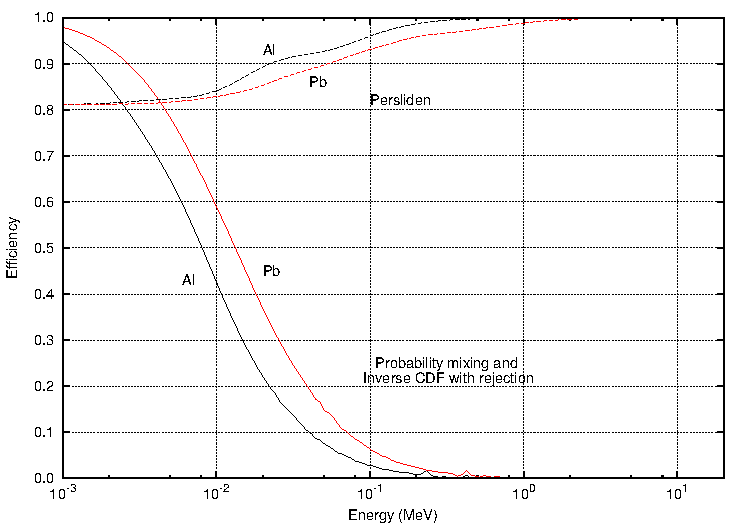
\includegraphics{chapters/photon_interactions/Persliden_experimental_sampling_method_eff.pdf}}
  \end{center}
  \caption{\textbf{Differential coherent cross section sampling procedure efficiencies.}
    \textit{The efficiency of the probability mixing and inverse CDF sampling 
      method with the atomic form factor rejection function and the efficiency 
      of Persliden's sampling method is shown for energies between one keV and 
      twenty MeV. Persliden's method is far superior as it has a high 
      efficiency at all energies.}}
  \label{fig:diff_coh_sampling_proc_eff}
\end{figure}

\section{Pair Production}
\label{sec:pair_production}
Pair production occurs when the photon interacts with the electric field of an
atom (screened nuclear field) producing an electron-positron pair. It can be
subdivided into two separate phenomemon depending on the state of the atom
after the interaction \citep{hubbell_pair_1980}. Coherent pair production occurs
when the entire atom recoils from the interaction without any internal 
excitation. Incoherent pair production occurs when the atom is left in an 
excited or ionized state. Pair production resulting in the ionization of an 
atom is often called triplet production because three outgoing particles (two 
electron and one positron) result from the interaction. However, triplet 
production is often used to refer to incoherent pair production (excitation and
ionization). 

The threshold for coherent pair production is $2m_ec^2$. The threshold for 
incoherent pair production is only slightly higher than the threshold for 
coherent pair production \citep{hubbell_pair_1980}. This is significantly 
different than the threshold for pair production in the field of a free 
electron (triplet production), which is $4m_ec^2$. However, the cross section 
for incoherent pair production below $4m_ec^2$ is very small and is usually 
neglected in data tables \citep{hubbell_pair_1980}. 

When one is conducting coupled photon-electron transport, the energy and 
direction of the outgoing electron and positron must be sampled. This can
be done using the Bethe-Hetler expression for the coherent pair production
cross section \citep{mukhin_experimental_1987, salvat_physics_2001}. This
cross section and the methods for sampling from it will be discussed in 
section \ref{}. When one is only interested in the transport of photons in 
the system, the pair production cross section can be formulated differently. 
Several assumptions will be made in the formulation of this approximate
cross section. The first is that the electron and positron deposit all of 
their energy locally (they stop immediately after being created). Since the 
mean free paths of electrons is generally much smaller than photons, this
assumption is usually acceptable. The second is that the positron will only
annihilate once its kinetic energy is essentially zero. In other words, the
annihilation of positrons in flight will be neglected. This results in a very
simple (isotropic) angular distribution of the annihilation photons. The final 
approximation is that the directions of the resulting annihilation photons are 
uncorrelated with the initial photon direction. Because of the tortorous path 
taken by a typical electron or positron, this approximation is usually 
acceptable as well. The simplified treatment allows the pair production and 
triplet production cross sections to be combined into a single cross section. 
The resulting double differential pair production is as follows 
\citep{hoogenboom_adjoint_2000,gabler_amos_2006}.
\begin{equation}
  \frac{d^2\sigma_{p.p.}(E^{'},Z)}{d\Omega dE} = \frac{2 [\sigma_{p.p.}(E^{'},Z) 
    + \sigma_{t.p.}(E^{'},Z)] \delta(E - m_ec^2)}{4\pi}
\end{equation}
Note that the double differential pair production cross section contains the 
factor two to denote that two photons are created from the reaction. 

As discuss in chapter \ref{ch:particle_transport} a single outgoing photon can
be followed as long as its weight is multiplied by two. Otherwise two photons
must be followed. Both outgoing photons will have an outgoing energy equal to
$m_ec^2$ as indicated by the delta function in the pair production cross 
section. The first photon will then have its outgoing direction sampled from
an isotropic distribution. The direction of the second photon will then simply
be the opposite direction of the first photon in accordance with conservation
of momentum (and under the assumption that the positron-electron pair that
annihilated had negligable momentum).

\section{The Photoelectric Effect}
The photoelectric effect occurs when a photon of energy E is absorbed by a
target atom, which makes a transition to an excited state or becomes ionized.
When ionization occurs, the ejected electron will have energy equal to the 
absorbed photon minus the binding energy of the electron. Atomic relaxation
will occur after the vacancy has been created. This process results in the 
emission of Auger electrons and x-rays. The x-rays may be of significance to
low energy photon simulations, especially when high atomic number elements are
present. It is therefore necessary to conduct a more detailed treatment of the
photoelectric effect in photon transport codes. Salvat et al. recommended a 
procedure in which only the K and L shells are treated in a detailed way
\citep{salvat_physics_2001}. The outer shells are treated together. The PDF
for selecting the shell containing the electron that is ejected is as follows.
\begin{align}
  p(i) = 
  \begin{cases}
    \frac{\sigma_{i,pe}(E^{'},Z)}{\sigma_{pe}(E^{'},Z)} & \text{for K, L1, L2 or L3 shells} \\
    1 - p_K - p_{L1} - p_{L2} - p_{L3} & \text{o.w.}
  \end{cases}
\end{align}

When ionization occurs in the K or L shell, the energy of the ejected electron
is equal to the energy of the photon minus the binding energy of the particular
shell. While this is also true for the outer shells, the binding energies are
small enough that they can be neglected. If coupled photon-electron transport
is not being conducted than all emitted electrons are ignored. When the K or
L shells become ionized, the subsequent atomic relaxation has the possibility
to result in the emission of x-rays with energy that can be significant
depending on the calculation being done and must therefore be simulated. The
emission of particles from atomic relaxation resulting from vacancies in the
outer shells will always be ignored because of the low energy of these 
particles. The direction of all particles emitted from the relaxation process
should be sampled from an isotropic distribution \citep{salvat_physics_2001}.

\section{Photonuclear Absorption}
Photonuclear absorption occurs when a gamma ray is absorbed by the nucleus of
an atom resulting in the emission of one or more neutrons, charged particles or
additional gamma rays. These reactions generally have small cross-sections
and are usually neglected in photon transport codes. However, the cross sections
do exhibit broad resonances in the 12 to 24 MeV energy range 
\citep{lux_monte_1991}. For high energy coupled neutron-photon transport this
interaction can be important to include. 

\section{Other Interactions}
There are many more interactions that can occur between a photon and an atom.
These processes include Delbr\"{u}ck scattering, Raman scattering\footnote{Raman scattering is an inelastic scattering process that leaves the target atom in an excited state instead of ionized \citep{cullen_epdl97_1997}.}, and 
photomeson production. All of these interactions contribute less than 1\% to the
total cross section and are therefore neglected \citep{lux_monte_1991}.

\section{Adjoint Incoherent Scattering}
To simulate adjoint incoherent scattering the differential adjoint incoherent 
scattering cross section must be derived. The mechanics of the interaction will
be the same, except that they will proceed in reverse. In other words, an
electron and photon will now interact at a point resulting in a single outgoing
photon of higher energy. As mentioned previously, electron transport will be
ignored so the electron will be ignored in the process. The collision mechanics,
assuming that the adjoint photon interacts with a stationary free electron are
described in the following equation.
\begin{equation}
  E = \frac{E^{'}}{1-\alpha^{'}(1-\cos{\theta})}
\label{eq:adjoint_energy_angle_relation}
\end{equation}
This equation can be found by solving equation 
\ref{eq:compton_scattering_energy_rel} for the incoming energy (and switching
primed variables). This equation is interesting in that it exhibits a 
discontinuity when 
\begin{equation}
  \cos{\theta} = 1 - \frac{1}{\alpha^{'}}
\end{equation}
Any value of $\cos{\theta}$ less than the above value will result in nonphysical
(negative) energies. Acceptable values of $\cos{\theta}$ that approach the 
above value will result in very large outgoing adjoint photon energies. 

Because of the discontinuity in the equation for the outgoing adjoint photon
energy, the adjoint Compton scattering process is bound by a minimum scattering
angle and not a minimum energy. The minimum angle is shown in the following 
equation. The variable $\mu$ represents the cosine of the polar scattering 
angle.
\begin{equation}
  \mu_{min} = 
  \begin{cases}
    -1 & \text{if } \alpha^{'} < \frac{1}{2} \\
    1 - \frac{1}{\alpha^{'}} & \text{if } \alpha^{'} \geq \frac{1}{2} 
  \end{cases}
\end{equation}
The maximum angle cosine is still unity.

The adjoint differential incoherent scattering cross section must now be 
derived using the definition of the adjoint cross section from equations
\ref{eq:adjoint_double_diff_transfer_prob} and \ref{eq:adjoint_cross_section}.
Note that the incoherent scattering cross section is independent of the photons
initial direction. In addition, the outgoing energy and outgoing direction
cosine are coupled. Therefore, the incoherent scattering process can be 
completely characterized by a differential scattering cross section in outgoing
energy only. 
\begin{align}
  \sigma_{i.s.}^{\dagger}(E^{'} \to E) & = \sigma_{i.s.}(E \to E^{'}) \nonumber \\
  \frac{d\sigma_{i.s.}^{\dagger}(E^{'},E,Z)}{dE} & = 
  \frac{d\sigma_{i.s.}(E,E^{'},Z)}{dE^{'}}
  \label{eq:adjoint_forward_cross_sec_rel}
\end{align}

The incoherent scattering cross section differential in outgoing energy is 
shown below. 
\begin{equation}
  \frac{d\sigma_{i.s.}(\alpha^{'},\alpha,Z)}{dE} = 
  \frac{\pi r_e^2}{m_ec^2 \alpha^{'2}}
  \left[\frac{\alpha}{\alpha^{'}} + \frac{\alpha^{'}}{\alpha} - 1 + cos^2\theta
    \right] S(y,Z)
\end{equation}
From this equation, the adjoint differential incoherent scattering cross section
is the following. To construct this equation, all of the primed and unprimed 
variables in the previous equation are switched in accordance with equation
\ref{eq:adjoint_forward_cross_sec_rel}. 
\begin{equation}
  \frac{d\sigma_{i.s.}^{\dagger}(\alpha^{'},\alpha,Z)}{dE} = 
  \frac{\pi r_e^2}{m_ec^2 \alpha^{2}}
  \left[\frac{\alpha^{'}}{\alpha} + \frac{\alpha}{\alpha^{'}} - 1 + cos^2\theta
    \right] S(y,Z)
  \label{eq:diff_adjoint_incoh_scatt_cross_sec_energy}
\end{equation}
It must also be noted that the first argument of the scattering function is
now $y = \sin{\frac{\theta}{2}}/\lambda$, which is dependent on the outgoing
photon wavelength.

A PDF for the outgoing energy can now be created, which will have a similar
form to the PDF from equation \ref{eq:incoherent_sampling_pdf}.
\begin{align}
  p^{\dagger}(\alpha|\alpha^{'},Z) & = \frac{1}{\sigma_{i.s.}^{\dagger}(\alpha^{'},Z)}
  \frac{d\sigma_{i.s.}^{\dagger}(\alpha^{'},\alpha,Z)}{dE} \nonumber \\
  & = \frac{S_{max}(y,Z)\sigma_{K.N.}^{\dagger}(\alpha^{'})}
       {\sigma_{i.s.}^{\dagger}(\alpha^{'},Z)} 
       \left[\frac{S(y,Z)}{S_{max}(y,Z)}\right]
       \left[\frac{1}{\sigma_{K.N.}^{\dagger}(\alpha^{'})}
         \frac{d\sigma_{K.N.}^{\dagger}(\alpha^{'},\alpha)}{dE}\right] \nonumber \\
  & = C^{\dagger}(\alpha^{'},Z)R(y,Z)p_{K.N.}^{\dagger}(\alpha|\alpha^{'})
  \label{eq:adj_incoherent_sampling_pdf}
\end{align}
Now, one samples an outgoing energy from the PDF 
$p_{K.N.}^{\dagger}(\alpha|\alpha^{'})$. This energy is either accepted or rejected
based on the rejection function $R(y,Z)$.

Using a similar change of variables to the one done for the differential 
Klein-Nishina cross section, the differential adjoint Klein-Nishina cross 
section can be written in terms of an inverse energy gain ratio.
\begin{align}
  \frac{1}{x} & = \frac{\alpha}{\alpha^{'}} \\
  x & = 1 - \alpha^{'}(1-\cos{\theta})
\end{align}
The differential adjoint Klein-Nishina cross section can then be written as 
follows (see Appendix \ref{ch:appendix_B}).
\begin{align}
  \frac{d\sigma_{K.N.}^{\dagger}(\alpha^{'},x)}{dx} & = 
  K^{\dagger}\left[A^{\dagger}x^2 + B^{\dagger}x
    + C^{\dagger} + \frac{D^{\dagger}}{x} \right] \\
  K^{\dagger} & = \frac{\pi r_e^2}{\alpha^{'}} \nonumber \\
  A^{\dagger} & = \frac{1}{\alpha^{'2}} \nonumber \\
  B^{\dagger} & = 1 + \frac{2(\alpha^{'}-1)}{\alpha^{'2}} \nonumber \\
  C^{\dagger} & = \frac{1-2\alpha^{'}}{\alpha^{'2}} \nonumber \\
  D^{\dagger} & = 1 \nonumber 
\end{align}

Now, a PDF for x can be created if the differential adjoint Klein-Nishina cross
section is divided by the total adjoint Klein-Nishina cross section. The total
adjoint Klein-Nishan cross section can be found by integrating the differential
Klein-Nishina cross section from $x_{min} = 1-\alpha^{'}(1-\mu_{min})$ to 
$x_{max} = 1$. Unfortunately, when the initial energy of the adjoint photon is
greater than $\frac{1}{2}m_ec^2$, the total adjoint Klein-Nishina cross section
will be infinite. The cross section can be bounded if a maximum energy is set, 
which is an acceptable requirement since every physical problem will have a 
maximum source energy. Associated with this maximum energy will be a new 
minimum scattering angle cosine and consequently a new minimum inverse energy 
gain ratio. 
\begin{equation*}
  \alpha_{max} = \frac{\alpha^{'}}{1-\alpha^{'}(1-\mu_{min})} \nonumber \\
\end{equation*}
\begin{align}
  \mu_{min} & = 
  \begin{cases}
    -1 & \text{if } \alpha^{'} < \frac{\alpha_{max}}{1+2\alpha_{max}} \\
    1 - \frac{1}{\alpha^{'}} + \frac{1}{\alpha_{max}} 
    & \text{if } \alpha^{'} \geq \frac{\alpha_{max}}{1+2\alpha_{max}} \\ 
  \end{cases} \\
  x_{min} & = 
  \begin{cases}
    1-2\alpha^{'} & \text{if } \alpha^{'} < \frac{\alpha_{max}}{1+2\alpha_{max}} \\
    \frac{\alpha^{'}}{\alpha_{max}} & \text{if } \alpha^{'} \geq
    \frac{\alpha_{max}}{1+2\alpha_{max}} \\
  \end{cases}
\end{align}

The PDF for x can be defined as follows.
\begin{align}
  p_{K.N.}^{\dagger}(x|\alpha^{'},\alpha_{max}) & = 
  \begin{cases}
    H^{\dagger}\left[A^{\dagger}x^2 + B^{\dagger}x + C^{\dagger} + \frac{D^{\dagger}}{x}
      \right] & \text{if } x_{min} \leq x \leq 1 \\
    0 & \text{o.w.}
  \end{cases} 
  \label{eq:adjoint_incoherent_pdf_x} \\
  H^{\dagger} & = \frac{K^{\dagger}}{\sigma_{K.N.}^{\dagger}(\alpha^{'},\alpha_{max})}
  \nonumber 
\end{align}
A direct inversion of this PDF is not possible. In addition, this PDF cannot be
sampled directly using a combination of the probability mixing method and the
inverse CDF method. If one were to split the PDF into a part for each term, as
is done with the PDF associated with the differential Klein-Nishina cross
section, the probability of selecting each part must be positive for the method
to work. The probability of selecting the part containing the value $B^{\dagger}$
would only be positive when $\alpha^{'} \geq -1 + \sqrt{3}$. The probability of
selecting the part containing the value $C^{\dagger}$ would only be positive when
$\alpha^{'} \leq \frac{1}{2}$. These two constraints cannot be simultaneously
satisfied and therefore, the PDF cannot be sampled directly.

The best remaining option is to create a rejection sampling scheme. An 
effective rejection sampling scheme becomes apparent if one reorganizes the
PDF from equation \ref{eq:adjoint_incoherent_pdf_x}.
\begin{align}
  p_{K.N.}^{\dagger}(x|\alpha^{'},\alpha_{max}) & = 
  \begin{cases}
    H^{\dagger}\left[x + \frac{1}{x} - 1 + cos^2\theta \right] 
    & \text{if } x_{min} \leq x \leq 1 \\
    0 & \text{o.w.}
  \end{cases} \nonumber \\
  & = 
  \begin{cases}
    H^{\dagger}\left[\left(\frac{1}{x} - 1 \right) + \left(x\right) + 
      \left(cos^2\theta\right) \right] 
    & \text{if } x_{min} \leq x \leq 1 \\
    0 & \text{o.w.}
  \end{cases} \label{eq:reorganized_adjoint_KN_pdf}
\end{align}
This equation has been split into three separate terms, two of which can be 
sampled from directly to create a very efficient rejection sampling procedure.
The rejection sampling scheme is shown in figure 
\ref{fig:adjoint_KN_rejection_sampling}. Refer to appendix \ref{ch:appendix_B}
for a derivation of this rejection sampling scheme.
\begin{figure}[t!]
  \begin{center}
    \def\svgwidth{360bp}
    \input{chapters/photon_interactions/Adjoint_KN_sampling_method.pdf_tex}
  \end{center}
  \caption{\textbf{Adjoint K.N. Rejection Sampling Procedure}.
    \textit{This sampling procedure is used to sample a value of x from the
    differential adjoint Klein-Nishina cross section. One can use this sampling
    procedure at any incoming particle energy.}}
  \label{fig:adjoint_KN_rejection_sampling}
\end{figure}

As shown in figure \ref{fig:diff_adj_incoh_sampling_proc_eff} (specifically the 
free electron case), the efficiency of this rejection sampling procedure is very
good at all energies. At lower energies and larger atomic numbers, the rejection
function $R(y,Z)$, which characterizes electron binding, causes a large decrease
in the overall sampling procedure efficiency compared to the free electron case.
The overall sampling procedure efficiency is still very good though.
\begin{figure}[t!]
  \begin{center}
    \scalebox{1.0}{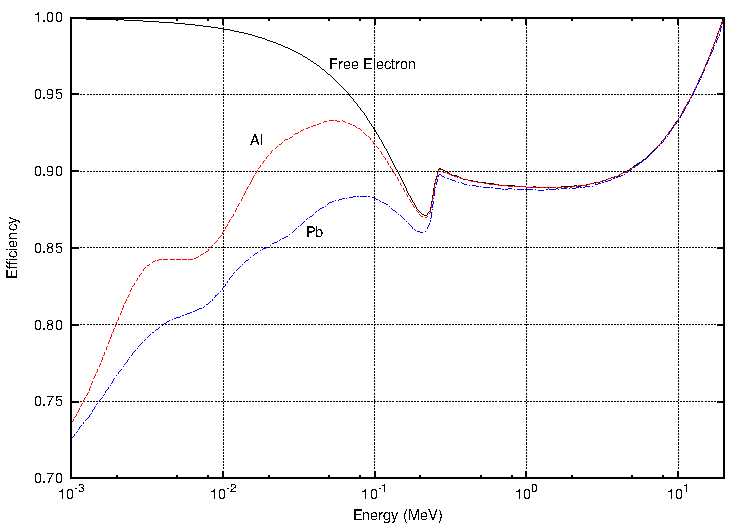
\includegraphics{chapters/photon_interactions/adjoint_KN_sampling_method_eff.pdf}}
  \end{center}
  \caption{\textbf{Differential adjoint incoherent cross section sampling procedure efficiencies.}
    \textit{The efficiency of the rejection sampling procedure for sampling 
      from the differential adjoint Klein-Nishina cross section with the 
      subsequent evaluation of the rejection function (based on the scattering 
      function) is shown for energies between one keV and twenty MeV. At lower 
      energies and higher atomic numbers, the rejection function has larger 
      effect on the sampling efficiency compared to the free electron case.}}
  \label{fig:diff_adj_incoh_sampling_proc_eff}
\end{figure}

To evaluate the adjoint weight factor, the adjoint incoherent cross 
section must be known. While this cross section is not provided in any of the
popular tables, it can be determined by integrating equation 
\ref{eq:diff_adjoint_incoh_scatt_cross_sec_energy} at an initial energy of
interest (or many to create a table). As indicated previously, the adjoint
incoherent cross section is a function of the maximum problem energy. Figure
\ref{fig:adjoint_incoh_cross_sec} shows the adjoint incoherent cross section 
for Aluminum as a function of initial energy and for three maximum problem 
energies: 1.0 MeV, 10.0 MeV and 20.0 MeV. As the maximum problem energy 
increases, the spike in the adjoint incoherent cross section centered at 
$\frac{\alpha_{max}}{1+2\alpha_{max}}$ increases. At the maximum problem energy, 
the adjoint incoherent cross section goes to zero.
\begin{figure}[t!]
  \begin{center}
    \scalebox{1.0}{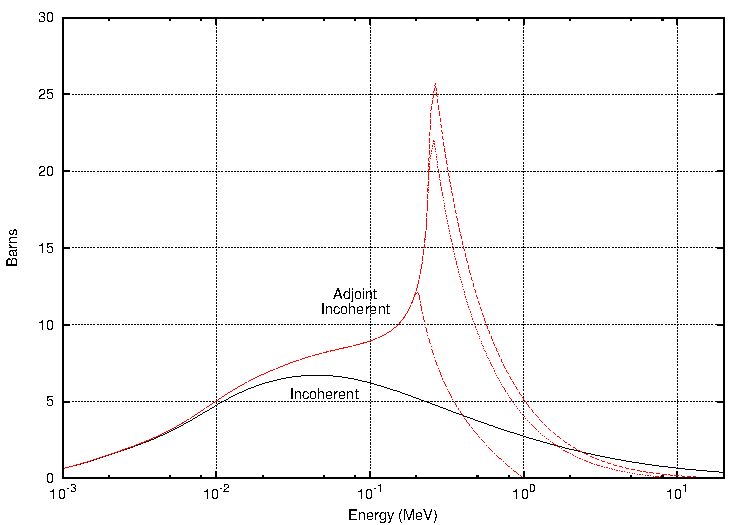
\includegraphics{chapters/photon_interactions/adjoint_and_forward_incoherent_cross_section-13.pdf}}
  \end{center}
  \caption{\textbf{Adjoint incoherent cross section for Aluminum.}
    \textit{The adjoint incoherent cross section evaluated at a maximum
      problem energy of 20.0 MeV, 10.0 MeV and 1.0 MeV is shown. As the 
      maximum problem energy increases, the spike in the adjoint incoherent
      cross section centered at $\frac{\alpha_{max}}{1+2\alpha_{max}}$ 
      increases. At the maximum problem energy, the cross section goes to 
      zero.}}
  \label{fig:adjoint_incoh_cross_sec}
\end{figure}

\section{Doppler Broadening of Incoherently Scattered Adjoint Photons}
In section \ref{sec:photon_dopp_broadening} doppler broadening of incoherently
scattered photons was discussed. While it hasn't been addressed in the 
literature yet, this process is also reversable. In this section, some 
arguments will be made to validate this claim. However, it must be noted that
no simulations have been completed yet to confirm the validity of this claim. 

In the derivation of the double differential incoherent scattering cross 
section, Ribberfors used the Born and impulse approximations. The impulse 
approximation is of particular importance because it allows the system to be
treated identically imediately before and imediately after the collision.
Therefore, the scattering mechanics using this approximation will be identical
for the adjoint process, except that they will happen in reverse. In addition,
the double differential incoherent scattering cross section is actually
differential in the incoming and outgoing photon energy difference 
\citep{cooper_compton_1985}. This variable will not change in the double 
differential adjoint incoherent scattering cross section despite the change in
primed and unprimed variables. Before presenting the double differential
adjoint incoherent scattering cross section, the adjoint incoherent scattering
cross section differential in steradians must be determined. A change of 
variables will be done using equations 
\ref{eq:diff_adjoint_incoh_scatt_cross_sec_energy} and 
\ref{eq:adjoint_energy_angle_relation}.
\begin{equation}
  \frac{d\sigma_{i.s.}^{\dagger}(\alpha^{'},\alpha,Z)}{d\Omega} = 
  \frac{r_e^2}{2}\left[\frac{\alpha^{'}}{\alpha} + \frac{\alpha}{\alpha^{'}} - 1
    + cos^2\theta \right]S(y,Z)
  \label{eq:diff_adjoint_incoh_cross_sec_steradian}
\end{equation}

Now, the double differential adjoint incoherent scattering cross section is
the following.
\begin{equation}
  \left(\frac{d\sigma^{\dagger}(\alpha^{'},\alpha,\theta,Z)}{d\Omega dE}
  \right)_i = \frac{r_e^2}{2c\left|\vec{\alpha}-\vec{\alpha^{'}}\right|}
  \left(\frac{\alpha^{'}}{\alpha}\right)\left(\frac{\alpha^{'}}{\alpha_c} +
  \frac{\alpha_c}{\alpha^{'}} - 1 + cos^2\theta \right) J_i(p_z,Z)
\end{equation}
The variable $\alpha_c$ is now the adjoint Compton line, which is the outgoing
adjoint photon energy in units of electron rest mass energy corresponding to
the outgoing scattering angle assuming that the electron upon which the adjoint
photon scattered was stationary and free (see equation 
\ref{eq:adjoint_energy_angle_relation}). The variable $p_z$ is still the 
electron momentum projection. However, the primed and unprimed variables in 
equation \ref{eq:pz} for $p_z$ are switched.
\begin{align}
  p_z & = m_ec \frac{\alpha^{'}-\alpha + \alpha\alpha^{'}(1-\cos{\theta})}
  {\left|\vec{\alpha}-\vec{\alpha^{'}}\right|} \nonumber \\
  & = m_ec \frac{\alpha^{'}-\alpha + \alpha\alpha^{'}(1-\cos{\theta})}
  {\sqrt{\alpha^2 + \alpha^{'2} - 2\alpha\alpha^{'}\cos{\theta}}} \nonumber
\end{align}

For the purposes of sampling from the double differential adjoint incoherent
cross section, it will again be more useful to do a change of variables from
outgoing energy to electron momentum projection $p_z$. The derivative of $p_z$
with respect to the outgoing adjoint photon energy is shown below.
\begin{equation}
  \frac{dp_z}{d\alpha} = m_ec\frac{-1 + \alpha^{'}(1-\cos{\theta})}
       {\left|\vec{\alpha}-\vec{\alpha^{'}}\right|} - 
       p_z\frac{\alpha-\alpha^{'}\cos{\theta}}
       {\left|\vec{\alpha}-\vec{\alpha^{'}}\right|^2}
\end{equation}
Using the same simplifications discussing in section 
\ref{sec:photon_dopp_broadening} this derivative can be approximated as
\begin{align}
  \frac{dp_z}{d\alpha} & = m_ec\frac{-1 + \alpha^{'}(1-\cos{\theta})}
       {\left|\vec{\alpha}-\vec{\alpha^{'}}\right|} \nonumber \\
   & = - \frac{m_ec \alpha^{'}}
       {\alpha_c\left|\vec{\alpha}-\vec{\alpha^{'}}\right|}
\end{align}
Now the change of variables in the double differential adjoint cross section
can be completed.
\begin{align}
  \left(\frac{d\sigma^{\dagger}(p_z,\theta,Z)}{d\Omega dp_z} \right)_i & = 
  \left(\frac{d\sigma^{\dagger}(\alpha^{'},\alpha,\theta,Z)}{d\Omega dE}
  \right)_i \frac{dE}{d\alpha} \left|\frac{d\alpha}{dp_z}\right| \nonumber \\
  & = \frac{r_e^2}{2} \left(\frac{\alpha_c}{\alpha}\right)
  \left(\frac{\alpha^{'}}{\alpha_c} + \frac{\alpha_c}{\alpha^{'}} - 1 + 
  cos^2\theta \right) J_i(p_z,Z)
\end{align}

The differential adjoint incoherent scattering cross section from equation
\ref{eq:diff_adjoint_incoh_cross_sec_steradian} can be recovered by integrating
over all possible electron momentum projections and by summing up the resulting
differential cross section for each shell. The approximation discussed in
section \ref{sec:photon_dopp_broadening} that $\alpha_c \approx \alpha$ will
be used again here to simplify the integral. The limit of integration
$p_{i,max}$ is the same as before. However, it will now occur when the outgoing
adjoint photon energy is equal to $E+E_{i,b}$, where $E_{i,b}$ is the binding
energy for the particular subshell. 
\begin{align}
  \frac{d\sigma_{i.s.}^{\dagger}(\alpha^{'},\theta,Z)}{d\Omega} & = 
  \frac{r_e^2}{2}\left[\frac{\alpha^{'}}{\alpha} + \frac{\alpha}{\alpha^{'}} - 1
    + cos^2\theta \right] \sum_i \int_{-\infty}^{p_{i,max}} J_i(p_z,Z)dp_z \nonumber\\
  & = \frac{d\sigma_{K.N.}^{\dagger}(\alpha^{'},\theta,Z)}{d\Omega} S^I(y,Z) 
  \nonumber \\
  & = \frac{d\sigma_{K.N.}^{\dagger}(\alpha^{'},\theta,Z)}{d\Omega} S(y,Z) 
  \nonumber
\end{align}
The fact that the differential adjoint incoherent cross section can be recovered
using similar approximations to the ones used to recover the differential 
incoherent cross section is a promising result, which adds credibility to the
claim that the photon doppler broadening process is reversible. 

A sampling method similar to the one proposed by Namito et al. for photon 
doppler broadening can now be created for adjoint photon doppler broadening. 
The first step is to sample an outgoing scattering angle from the differential
adjoint incoherent cross section using the rejection method from the 
previous section. Next, the subshell containing the electron upon which the
adjoint photon will scatter must be sampled. This will again be done by
creating a discrete PDF based on the number of electrons in each shell.
\begin{equation*}
  p(i) = \frac{n_i}{Z}
\end{equation*}
Finally, an outgoing adjoint photon energy must be sampled from the double
differential adjoint incoherent cross section. A conditional PDF for the 
outgoing photon energy can be created by dividing the double differential
adjoint incoherent cross section by the differential adjoint incoherent cross
section evaluated at a particular angle. The value of $p_{i,max}$ is 
calculated from the equation for $p_z$ using the value of $\theta$ that was 
sampled and the substitution $\alpha = \alpha^{'} + \frac{E_{i,b}}{m_ec^2}$.
\begin{align}
  p_i^{\dagger}(p_z|\theta,Z) & = 
  \left(\frac{d\sigma_{i.s.}^{\dagger}(\alpha^{'},\theta,Z)}{d\Omega}\right)_i^{-1}
  \left(\frac{d\sigma^{\dagger}(p_z,\theta,Z)}{d\Omega dp_z} \right)_i \nonumber\\
  & = \left(\frac{\alpha_c}{\alpha}\right)\frac{J_i(p_z,Z)}{S_i(y,Z)}
  \nonumber \\
  & = \left(\frac{1}{1-\alpha^{'}(1-\cos{\theta})}\right)
  \left(\frac{\alpha^{'}}{\alpha}\right) 
  \left(\frac{J_i(p_z,Z)}{\int_{-\infty}^{p_{i,max}}J_i(p_z,Z) dp_z}\right)
  \nonumber \\
  & = C^{\dagger}(\alpha^{'},\theta)R^{\dagger}(\alpha^{'},\alpha)p(p_z,Z)
\end{align}
One must sample a value of $p_z$ from the PDF $p(p_z,Z)$ to determine the
outgoing adjoint photon energy. The same table method discussed in section
\ref{sec:photon_dopp_broadening} can be used to sample a value of $p_z$ from
the PDF. Once the outgoing adjoint photon energy has been determined the 
rejection function $R(\alpha,\alpha^{'})$ is used to determine if the value 
should be accepted or rejected. 

The equation for the outgoing adjoint photon energy in terms of the momentum
projection is shown below. When both values are energetically possible, one of
the values must be randomly selected (with probability one half).
\begin{align}
  \alpha &= \frac{-b^{\dagger}}{2a^{\dagger}} \pm 
  \frac{\sqrt{b^{\dagger 2} - 4a^{\dagger}c^{\dagger}}}{2a^{\dagger}} \\
  a^{\dagger} & = \left(\frac{p_z}{m_ec}\right)^2 - 
  \left(\frac{\alpha^{'}}{\alpha_c}\right)^2
  \nonumber \\
  b^{\dagger} & = -2\alpha^{'}\left[\left(\frac{p_z}{m_ec}\right)^2\cos{\theta} + 
  \frac{\alpha^{'}}{\alpha_c}\right] \nonumber \\
  c^{\dagger} & = \alpha^{'2}\left[\left(\frac{p_z}{m_ec}\right)^2 - 1\right] 
  \nonumber
\end{align}

\section{Adjoint Coherent Scattering}
While it hasn't been stated explicitly, by neglecting photon polarization and
interference effects, which were limitations of the transport equation discussed
in chapter \ref{ch:particle_transport}, all of the differential photon cross
sections are independent of the direction of the photon. The coherent scattering
cross section is unique in that it is also independent of the outgoing photon
energy. Because the derivation of the differential adjoint cross sections 
involves the reversal of the incoming and outgoing energy as well as the 
incoming and outgoing direction, any differential cross section that is 
independent of both the outgoing energy and direction will be its own adjoint
cross section. Therefore, coherent scattering is identical for both photons and
adjoint photons. All of the techniques discussed in section 
\ref{sec:coherent_scattering} for sampling an outgoing direction from the 
differential coherent scattering cross section should be used with adjoint
photons.

\section{Adjoint Pair Production}
To simulate adjoint pair production the differential adjoint pair production 
cross section must be derived. This can be done using the definition of the
adjoint cross section from equations \ref{eq:adjoint_double_diff_transfer_prob} 
and \ref{eq:adjoint_cross_section}. The pair production cross section, which
was presented in \ref{sec:pair_production}, is independent of the photon's 
initial direction. Because the outgoing energy and direction are not coupled,
the dependence of the double differential adjoint pair production cross section 
on the outgoing direction relative to the incoming direction will be the same
as with the double differential pair production cross section.
\begin{align}
  \frac{d\sigma_{p.p.}^{\dagger}(E^{'} \to E)}{d\Omega} & = 
  \frac{d\sigma_{p.p.}(E \to E^{'})}{d\Omega} \nonumber \\
  \frac{d^2\sigma_{p.p.}^{\dagger}(E^{'},E,Z)}{d\Omega dE} & = 
  \frac{d^2\sigma_{p.p.}^{\dagger}(E,E^{'},Z)}{d\Omega dE^{'}}
\end{align}

The double differential adjoint pair production cross section is shown below
\citep{hoogenboom_adjoint_2000}.
\begin{equation}
  \frac{d^2\sigma_{p.p.}^{\dagger}(E^{'},E,Z)}{d\Omega dE} = 
  \frac{2\left[\sigma_{p.p.}(E,Z)+\sigma_{t.p}(E,Z)\right]\delta(E^{'}-m_ec^2)}
  {4\pi}
\end{equation}
Interestingly, the double differential adjoint pair production cross section
will be zero unless the initial energy of the photon is equal to the rest mass 
of the electron. Therefore, the adjoint pair production process will never be
sampled because the probability of an adjoint particle scattering into the
energy $m_ec^2$ exactly during a random walk is zero. This issue indicates that
the adjoint random walk process presented in chapter 
\ref{ch:adjoint_particle_transport} is insufficient for adjoint photons. A 
modified adjoint random walk process must be derived which will enable adjoint 
pair production reactions to occur. 

To start, recall the adjoint emission density FIESK.
\begin{equation*}
  \begin{split}
    \theta^{\dagger}(\vec{r},E,\hat{\Omega}) = a(\vec{r},E,\hat{\Omega}) + 
    \int\int&\int P^{\dagger}(\vec{r},E^{'})
    C^{\dagger}(\vec{r},E^{'} \to E,\hat{\Omega}^{'} \to \hat{\Omega}) \\
    & \cdot T^{\dagger}(\vec{r}^{'} \to \vec{r},E^{'},\hat{\Omega}^{'})
    \theta^{\dagger}(\vec{r}^{'},E^{'},\hat{\Omega}^{'})
    dV^{'} dE^{'} d\hat{\Omega}^{'}
  \end{split}
\end{equation*}
Using the definition of the adjoint collision density from equation 
\ref{eq:adj_collision_dens_to_adj_emission_dens}, the adjoint emission density
FIESK becomes
\begin{equation*}
    \theta^{\dagger}(\vec{r},E,\hat{\Omega}) = a(\vec{r},E,\hat{\Omega}) + 
    \int\int P^{\dagger}(\vec{r},E^{'})
    C^{\dagger}(\vec{r},E^{'} \to E,\hat{\Omega}^{'} \to \hat{\Omega})
    \xi^{\dagger}(\vec{r},E^{'},\hat{\Omega}^{'}) dE^{'} d\hat{\Omega}^{'}.
\end{equation*}
The adjoint weight factor and the adjoint collision kernel will now be expanded.
\begin{equation*}
    \theta^{\dagger}(\vec{r},E,\hat{\Omega}) = a(\vec{r},E,\hat{\Omega}) + 
    \int\int \sum_j \frac{\Sigma_j(\vec{r},E)c_j(\vec{r},E)
      f_j(E \to E^{'},\hat{\Omega} \to \hat{\Omega}^{'})}{\Sigma_T(\vec{r},E^{'})}
    \xi^{\dagger}(\vec{r},E^{'},\hat{\Omega}^{'}) dE^{'} d\hat{\Omega}^{'}.
\end{equation*}
The double differential adjoint pair production cross section will now be
pulled from the summation in the above equation creating a new term.
\begin{align}
  \theta^{\dagger}(\vec{r},E,\hat{\Omega}) & = a(\vec{r},E,\hat{\Omega}) 
  \nonumber \\
  & \quad + \int\int \sum_{j \neq p.p.} \frac{\Sigma_j(\vec{r},E)c_j(\vec{r},E)
    f_j(E \to E^{'},\hat{\Omega} \to \hat{\Omega}^{'})}{\Sigma_T(\vec{r},E^{'})}
  \xi^{\dagger}(\vec{r},E^{'},\hat{\Omega}^{'}) dE^{'} d\hat{\Omega}^{'}
  \nonumber \\ 
  & \quad + \frac{2\left[\Sigma_{p.p.}(\vec{r},E)+\Sigma_{t.p}(\vec{r},E)\right]}
  {4\pi} \int\int \frac{\delta(E^{'}-m_ec^2)}{\Sigma_T(\vec{r},E^{'})}
  \xi^{\dagger}(\vec{r},E^{'},\hat{\Omega}^{'}) dE^{'} d\hat{\Omega}^{'}
  \nonumber \\
  & = a(\vec{r},E,\hat{\Omega}) \nonumber \\
  & \quad + \int\int \frac{\Sigma_{i+c}^{\dagger}(\vec{r},E^{'})}
            {\Sigma_T(\vec{r},E^{'})} 
            \sum_{j \neq p.p.} \frac{\Sigma_j(\vec{r},E)c_j(\vec{r},E)
              f_j(E \to E^{'},\hat{\Omega} \to \hat{\Omega}^{'})}
                {\Sigma_{i+c}^{\dagger}(\vec{r},E^{'})}
            \xi^{\dagger}(\vec{r},E^{'},\hat{\Omega}^{'}) dE^{'} d\hat{\Omega}^{'}
            \nonumber \\ 
  & \quad + \frac{2\left[\Sigma_{p.p.}(\vec{r},E)+\Sigma_{t.p}(\vec{r},E)\right]}
                 {4\pi \Sigma_T(\vec{r},m_ec^2)}
  \int \xi^{\dagger}(\vec{r},m_ec^2,\hat{\Omega}^{'}) d\hat{\Omega}^{'}
  \nonumber \\
  & = a(\vec{r},E,\hat{\Omega}) \nonumber \\
  & \quad + \int\int P_{i+c}^{\dagger}(\vec{r},E^{'})
  C_{i+c}^{\dagger}(\vec{r},E^{'} \to E, \hat{\Omega}^{'} \to \hat{\Omega})
  \xi^{\dagger}(\vec{r},E^{'},\hat{\Omega}^{'}) dE^{'} d\hat{\Omega}^{'}
  \nonumber \\
  & \quad + \frac{2\left[\Sigma_{p.p.}(\vec{r})+\Sigma_{t.p}(\vec{r})\right]}
            {4\pi\Sigma_T(\vec{r},m_ec^2)}
  \frac{\left[\Sigma_{p.p.}(\vec{r},E)+\Sigma_{t.p}(\vec{r},E)\right]}
  {\left[\Sigma_{p.p.}(\vec{r})+\Sigma_{t.p}(\vec{r})\right]} 
  \int \xi^{\dagger}(\vec{r},m_ec^2,\hat{\Omega}^{'}) d\hat{\Omega}^{'}
  \nonumber \\
  & = a(\vec{r},E,\hat{\Omega}) \nonumber \\
  & \quad + \int\int P_{i+c}^{\dagger}(\vec{r},E^{'})
  C_{i+c}^{\dagger}(\vec{r},E^{'} \to E, \hat{\Omega}^{'} \to \hat{\Omega})
  \xi^{\dagger}(\vec{r},E^{'},\hat{\Omega}^{'}) dE^{'} d\hat{\Omega}^{'}
  \nonumber \\
  & \quad + \frac{1}{4\pi}P_{p.p.}^{\dagger}(\vec{r},m_ec^2)
  p_{p.p.}^{\dagger}(\vec{r},E)
  \int \xi^{\dagger}(\vec{r},m_ec^2,\hat{\Omega}^{'}) d\hat{\Omega}^{'}
  \nonumber 
\end{align}
The subscript (i+c) indicates that only incoherent and coherent scattering are
considered in the particular factor or kernel. 

As mentioned previously, the adjoint pair production cross section is zero 
except for when the incoming photon energy is exactly $m_ec^2$. Therefore, the 
following relations can be used to simplify the above equation. 
\begin{align}
  C_{i+c}^{\dagger}(\vec{r},E^{'} \to E, \hat{\Omega}^{'} \to \hat{\Omega}) & = 
  C^{\dagger}(\vec{r},E^{'} \to E, \hat{\Omega}^{'} \to \hat{\Omega}) \\
  P_{i+c}^{\dagger}(\vec{r},E^{'}) & = P^{\dagger}(\vec{r},E^{'})
\end{align}
\begin{align}
  \theta^{\dagger}(\vec{r},E,\hat{\Omega}) & = a(\vec{r},E,\hat{\Omega})
  \nonumber \\
  & \quad + \int\int\int P^{\dagger}(\vec{r},E^{'})
  C^{\dagger}(\vec{r},E^{'} \to E, \hat{\Omega}^{'} \to \hat{\Omega})
  T^{\dagger}(\vec{r}^{'} \to \vec{r},E^{'},\hat{\Omega}^{'})
    \theta^{\dagger}(\vec{r}^{'},E^{'},\hat{\Omega}^{'})
    dV^{'} dE^{'} d\hat{\Omega}^{'} \nonumber \\
  & \quad + \frac{1}{4\pi}P_{p.p.}^{\dagger}(\vec{r},m_ec^2)
  p_{p.p.}^{\dagger}(\vec{r},E)
  \int \xi^{\dagger}(\vec{r},m_ec^2,\hat{\Omega}^{'}) d\hat{\Omega}^{'}
  \nonumber 
\end{align}
The equation for the adjoint emission density is identical to the equation
presented in chapter \ref{ch:adjoint_particle_transport} except that there is
now an additional term. This additional term, which was missed in the initial
derivation, takes into account adjoint pair production. By manipulating this 
term further, the necessary modification to the adjoint random walk process
will become aparent. This term will temporarily be refered to as  $T_3$. 
The FIESK for the adjoint emission density, shown in equation 
\ref{eq:adj_collision_dens_fiesk} will now be substitued into $T_3$.
\begin{align}
  T_3 & = \frac{1}{4\pi}P_{p.p.}^{\dagger}(\vec{r},m_ec^2)
  p_{p.p.}^{\dagger}(\vec{r},E) 
  \int\int T^{\dagger}(\vec{r}^{'} \to \vec{r},m_ec^2,\hat{\Omega}^{'})
  a(\vec{r}^{'},m_ec^2,\hat{\Omega}^{'}) dV^{'}d\hat{\Omega}^{'} \nonumber \\
  & \quad + \frac{1}{4\pi}P_{p.p.}^{\dagger}(\vec{r},m_ec^2)
  p_{p.p.}^{\dagger}(\vec{r},E) \int\int\int\int
  T^{\dagger}(\vec{r}^{'} \to \vec{r},m_ec^2,\hat{\Omega}^{'})
  C^{\dagger}(\vec{r},E^{''} \to m_ec^2, \hat{\Omega}^{''} \to \hat{\Omega}^{'})
  \nonumber \\
  & \qquad \qquad \qquad \qquad \qquad \qquad \qquad \qquad \cdot
  P^{\dagger}(\vec{r}^{'},E^{''}) \xi^{\dagger}(\vec{r}^{'},E^{''},\hat{\Omega}^{''}) 
  dE^{''}d\hat{\Omega}^{''}dV^{'}d\hat{\Omega}^{'}
  \nonumber 
\end{align}
A new kernel will now be introduced, which is specific to adjoint pair 
production.
\begin{equation}
  O_{p.p.}^{\dagger}(\vec{r}^{'} \to \vec{r}, m_ec^2 \to E, \hat{\Omega}^{'}
  \to \hat{\Omega}) = \frac{1}{4\pi}P_{p.p.}^{\dagger}(\vec{r},m_ec^2)
  p_{p.p.}^{\dagger}(\vec{r},E) 
  T^{\dagger}(\vec{r}^{'} \to \vec{r},m_ec^2,\hat{\Omega}^{'})
\end{equation}
The equation for $T_3$ then becomes the following. The kernel $M^{\dagger}$,
defined in equation \ref{eq:adj_emission_dens_kernel}, is specific to the 
adjoint emission density.
\begin{align}
  T_3 & = \int\int 
  O_{p.p.}^{\dagger}(\vec{r}^{'} \to \vec{r}, m_ec^2 \to E, \hat{\Omega}^{'}
  \to \hat{\Omega}) a(\vec{r}^{'},m_ec^2,\hat{\Omega}^{'}) 
  dV^{'}d\hat{\Omega}^{'} \nonumber \\
  & \quad + \int\int 
  O_{p.p.}^{\dagger}(\vec{r}^{'} \to \vec{r}, m_ec^2 \to E, \hat{\Omega}^{'}
  \to \hat{\Omega}) \int\int\int
  M^{\dagger}(\vec{r^{''}} \to \vec{r}^{'},E^{''} \to m_ec^2,\hat{\Omega^{''}} \to 
  \hat{\Omega}^{'}) \nonumber \\
  & \qquad\qquad\qquad\cdot
  \theta^{\dagger}(\vec{r}^{''},E^{''},\hat{\Omega}^{''}) 
  dV^{''}dE^{''}d\hat{\Omega}^{''}dV^{'}d\hat{\Omega}^{'}
  \label{eq:pair_production_term}
\end{align}
The first term of $T_3$ is a new source term that accounts for adjoint particle 
emission from the adjoint source with energy exactly equal to the rest mass 
energy of the electron. The second term forces adjoint particles to 
scatter into the energy $m_ec^2$ whenever energetically possible at which point
adjoint pair production can occur.

The modified random walk procedure is now completely defined by the third
term of the adjoint emission density FIESK. The first modification is that 
the starting state of the adjoint particle must be sampled from either the 
adjoint source or the new source, which is shown below.
\begin{equation}
  S_{p.p.}^{\dagger}(\vec{r},m_ec^2,\hat{\Omega}) =
  \int\int O_{p.p.}^{\dagger}(\vec{r}^{'} \to \vec{r}, m_ec^2 \to E, \hat{\Omega}^{'}
  \to \hat{\Omega}) a(\vec{r}^{'},m_ec^2,\hat{\Omega}^{'}) 
  dV^{'}d\hat{\Omega}^{'}
\end{equation}
Sampling from this source will be done indirectly. Assume that the adjoint
source has the following form.
\begin{equation*}
  a(\vec{r},E,\hat{\Omega}) = f_{\vec{r}}(\vec{r})f_E(E)
  f_{\hat{\Omega}}(\hat{\Omega})
 \end{equation*}
The PDF for selecting a particular starting energy is then the following.
\begin{equation*}
  p_E(E) = \frac{f_E(E)}{\int f_E(E^{'})dE^{'}}
\end{equation*}
Because every particle will be emitted from the new source with energy
$m_ec^2$, the particles initial weight must be $p_E(m_ec^2)$. Next, a new
position is sampled from the adjoint transport kernel. Then the weight of the 
particle is multiplied by the adjoint pair production weight factor. Finally, 
an outgoing energy is sampled from the adjoint pair production kernel. The
last two steps will be discussed more shortly.

The next modification to the random walk process occurs when indirectly 
sampling from the adjoint collision kernel. If adjoint incoherent scattering is 
selected and it is energetically possible for the adjoint particle to 
scattering into the energy $m_ec^2$, a new random walk is initiated. The weight 
of this new random walk will be the weight of the initial random walk times the 
probability of scattering to the energy $m_ec^2$.
\begin{equation}
  W = W_m p_{i.s.}^{\dagger}(E^{'} \to m_ec^2)
\end{equation}
Given the properties of the adjoint incoherent scattering process, it will
only be energetically possible for an adjoint photon to scatter into the
energy $m_ec^2$ if its energy is in the following range.
\begin{equation}
  \frac{1}{3} \leq \alpha^{'} \leq 1
\end{equation}
Next, a new position is sampled from the adjoint transport kernel. At the
new collision point, the weight of the adjoint photon is multiplied by the 
adjoint pair production weight factor, which is defined below. As with the
adjoint incoherent cross section, where a maximum problem energy must be set in
order to keep the cross section finite, a maximum problem energy must also be 
set in order to keep the adjoint pair production weight factor finite. 
\begin{align}
  P_{p.p.}^{\dagger}(\vec{r},m_ec^2) & = 
  \frac{2\left[\Sigma_{p.p.}(\vec{r})+\Sigma_{t.p}(\vec{r})\right]}
       {\Sigma_T(\vec{r},m_ec^2)} \\
  \Sigma_{p.p.}(\vec{r}) & = \int_{2m_ec^2}^{E_{max}}\Sigma_{p.p.}(\vec{r},E)dE \\
  \Sigma_{t.p.}(\vec{r}) & = \int_{4m_ec^2}^{E_{max}}\Sigma_{t.p.}(\vec{r},E)dE
\end{align}
Finally an outgoing energy is sampled from the PDF present in the adjoint
pair production kernel. As with the the adjoint collision kernel, the 
PDF present in the adjoint pair production kernel will be sampled indirectly.
\begin{align}
  p_{p.p.}^{\dagger}(\vec{r},E) & = 
  \frac{\Sigma_{p.p.}(\vec{r},E)+\Sigma_{t.p}(\vec{r},E)}
  {\Sigma_{p.p.}(\vec{r})+\Sigma_{t.p}(\vec{r})} \nonumber \\
  & = \frac{\Sigma_{p.p.}(\vec{r},E)}
  {\Sigma_{p.p.}(\vec{r})+\Sigma_{t.p}(\vec{r})} +
  \frac{\Sigma_{t.p.}(\vec{r})}
  {\Sigma_{p.p.}(\vec{r})+\Sigma_{t.p}(\vec{r})} \nonumber \\
  & = \frac{\Sigma_{p.p.}(\vec{r})}
  {\Sigma_{p.p.}(\vec{r})+\Sigma_{t.p}(\vec{r})} 
  \frac{\Sigma_{p.p.}(\vec{r},E)}{\Sigma_{p.p.}(\vec{r})} +
  \frac{\Sigma_{t.p.}(\vec{r})}
  {\Sigma_{p.p.}(\vec{r},E)+\Sigma_{t.p}(\vec{r},E)}
  \frac{\Sigma_{t.p.}(\vec{r},E)}{\Sigma_{t.p.}(\vec{r})} \nonumber \\
  & = p_{p.p.}^{\dagger}(\vec{r}) \sum_A
  \frac{\Sigma_{p.p.,A}(\vec{r})}{\Sigma_{p.p.,A}(\vec{r})}
  \frac{\sigma_{p.p.,A}(E)}{\sigma_{p.p.,A}} +
  p_{t.p.}^{\dagger}(\vec{r}) \sum_A
  \frac{\Sigma_{t.p.,A}(\vec{r})}{\Sigma_{t.p.,A}(\vec{r})}
  \frac{\sigma_{t.p.,A}(E)}{\sigma_{t.p.,A}} \nonumber \\
  & = \sum_{i=1}^2 p_i^{\dagger}(\vec{r})\sum_A p_{i,A}^{\dagger}(\vec{r})
  p_{i,A}^{\dagger}(E)
\end{align}
Now, either the pair production or the triplet production distribution will
be sampled from by selecting from the discrete PDF $p_i^{\dagger}(\vec{r})$. The
value of $i$ sampled will determine which distribution is used. Next, an 
element hit will be sampled from the discrete PDF $p_{i,A}^{\dagger}(\vec{r})$. 
Finally, an outgoing energy is sampled from the continuous PDF 
$p_{i,A}^{\dagger}(E)$. Once the outgoing energy has been chosen, this random 
walk will continue normally.

\section{Discrete Energy Sources and Adjoint Photon Random Walks}
For sources with discrete energies, the energy point detector described in
chapter \ref{ch:adjoint_particle_transport} must be used. Assume that the
source is defined as follows.
\begin{equation}
  S(\vec{r},E,\hat{\Omega}) = 
  \begin{cases}
    S_0 \sum_i p_i \delta(E - E_{s,i}) p_{s,\hat{\Omega}}(\hat{\Omega})
    p_{s,\vec{r}}(\vec{r}) & \text{if } \vec{r} \in V_s \\
    0 & \text{o.w.}
  \end{cases}
\end{equation}
The only reaction for adjoint photons that can change the particles energy 
(given any initial energy) is adjoint incoherent scattering. Therefore,
as required by the energy point detector, every time an adjoint incoherent
scattering event is selected and the adjoint photon's energy is in the 
necessary energy window, an additional random walk must be initiated. The
weight assiciated with this new random walk will be the weight of the main
random walk times the probability of incoherently scattering from the current 
energy to the source energy.
\begin{align}
  W & = W_m p_{A,i.s.}^{\dagger}(\alpha_{s,i}|\alpha^{'},Z) \nonumber \\
  & = \frac{W_m}{\sigma_{A,i.s.}(\alpha^{'},Z)}
  \frac{d\sigma_{A,i.s.}^{\dagger}(\alpha^{'},\alpha,Z)}{dE}\Big|_{E_{s,i}}
\end{align}
The PDF from equation \ref{eq:adj_incoherent_sampling_pdf} is shown in the 
above equation. The outgoing direction cosine is directly coupled to the 
initial and outgoing energy. 
\begin{equation}
  \mu_{s,i} = 1 + \frac{1}{\alpha_{s,i}} - \frac{1}{\alpha^{'}}
\end{equation}
The outgoing azimuthal angle is simply sampled from a uniform distribution
over the interval (0,$2\pi$). 

The necessary energy window for possible scattering into each discrete source
energy is the following.
\begin{equation}
  \frac{\alpha_{s,i}}{1+2\alpha_{s,i}} \leq \alpha^{'} \leq \alpha_{s,i}
\end{equation}
When the adjoint photon energy is in a region where two or more energy windows
overlap, the energy point detector will be used with each source energy
associated with the windows. This means that more than one additional random
walk can be split off at each collision point because of the energy point
detector. 

The uncollided contribution to the inner product of interest must
also be estimated using the procedure that was outlined in chapter 
\ref{ch:adjoint_particle_transport}. 

\section{The Adjoint Weight Factor for Photons}
As described in chapter \ref{ch:adjoint_particle_transport}, after an adjoint
photon has been transported to the next collision site the weight must be 
multiplied by the adjoint weight factor. Because the adjoint weight factor
is the ratio of the total macroscopic adjoint cross section to the total
macroscopic cross section, it is not bound to the interval (0,1) but instead
to the interval (0,$\infty$). The adjoint weight factor will therefore have the
potential to negatively affect the variance of the estimators used. By examining
the adjoint weight factor for photons, the severity of the problem can be 
estimated. Figure \ref{fig:adjoint_weight_factor} shows the adjoint weight 
factor for aluminum and lead with a maximum problem energy of 20.0 MeV. 
Interestingly, the problem is much less severe for lead since the adjoint 
weight factor only goes above unity for a small range of energies. In addition
the maximum value of the adjoint weight factor for lead is much smaller than
for aluminum. The true effect that the adjoint weight factor has on the 
variance of the estimator used can only be evaluated by running example 
problems.
\begin{figure}[t!]
  \begin{center}
    \scalebox{1.0}{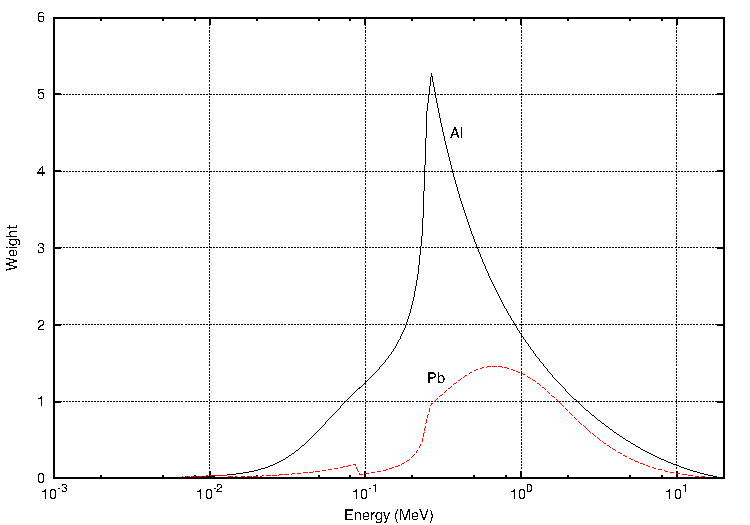
\includegraphics{chapters/photon_interactions/adjoint_weight_factor.pdf}}
  \end{center}
  \caption{\textbf{The adjoint weight factor for Aluminum and Lead.}
    \textit{The adjoint weight factor for Aluminum and Lead is shown for a
      maximum problem energy of 20.0 MeV. The adjoint weight factor for 
      Aluminum is more problematic than the adjoint weight factor for Lead
      since it has a higher maximum value and a larger range of energies where
      it is above unity.}}
  \label{fig:adjoint_weight_factor}
\end{figure}
